\section*{Multi-Carrier and OFDM Technologies}






La tecnologia multi-carrier è impiegata da tutte le modulazioni più recenti e rappresenta la base del livello fisico per trasmissioni LTE, 5G e Wi-Fi. 
L'ampio utilizzo di questa tiplogia di modulazione deriva dalla capacità di ridurre i problemi derivanti dall'utilizzo di un canale frequency selective, i cui problemi sono sempre più evidenti all'aumentare del rate di trasmissione. Inoltre presenta dei benefici anche nell'occupazione spetrale e nella flessibilità di allocazione delle risorse radio ai vari utenti del sistema.
\begin{itemize}
    \item Robustezza contro canali frequecy-selective
    \item Efficienza spettrale
    \item Allocazione flessibile di risorse
\end{itemize}

L'idea base consiste nel suddividere il segnale originale da trasmettere, caratterizzato da una banda ben superiore rispetto alla coherence bandwidth del canale in tanti segnali, ciascuno avente una banda tale da evitare i problemi del canale frequency selective, oveero inferiori alla coherence bandwidth.





\begin{center}
    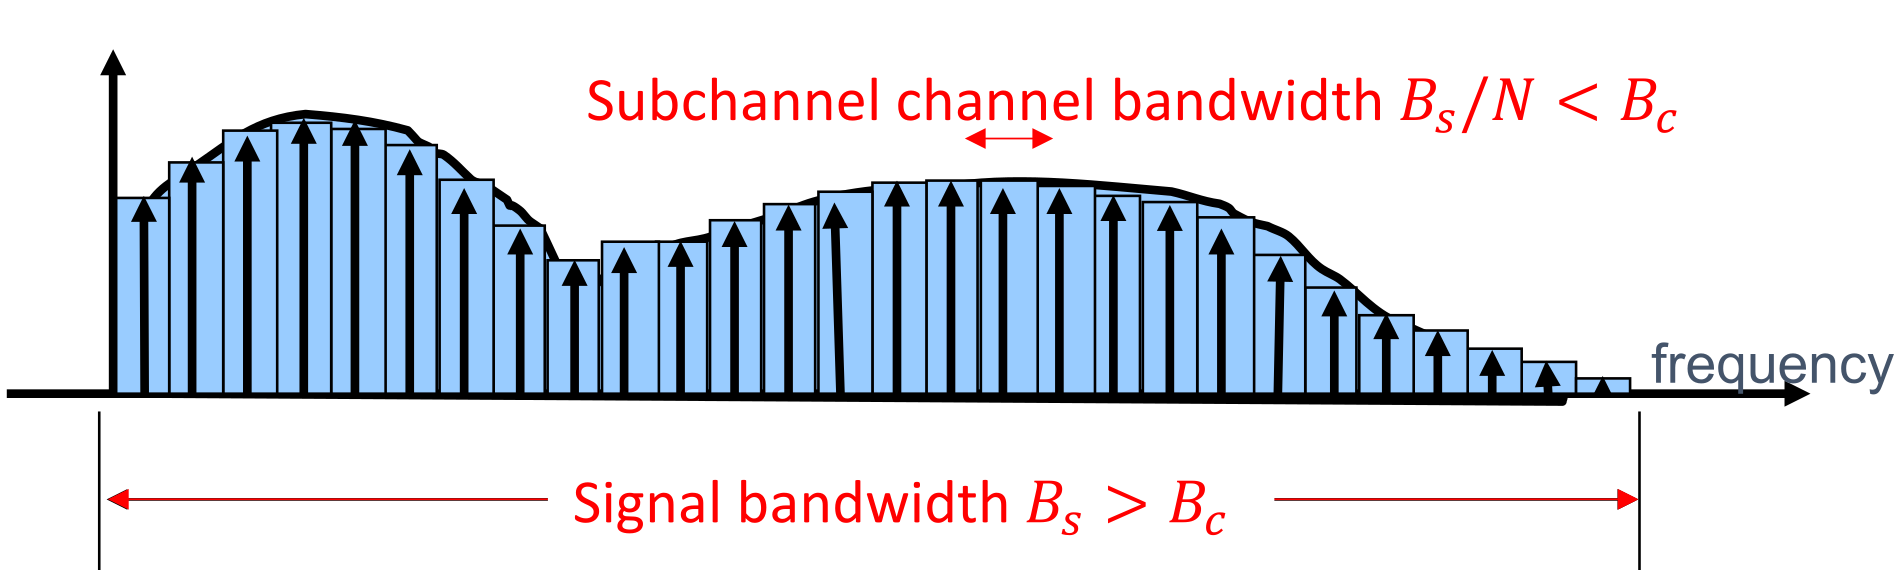
\includegraphics[width=0.8\textwidth]{imgs/multicarrier.jpg}
\end{center}
 



\[
  B_s > B_c \Rightarrow \text{frequency selective channel}  
\]

\[
    \Delta B = \frac{B_s}{N} < B_c \Rightarrow \text{flat fading channel}
\]
I segnali in cui è stato suddiviso l'originale non saranno affetti da ISI.

Per effettuare una trasmissione parallela dei veri segnali si potrebbe utilizzare filtri passa banda in parallelo, tuttavia nella pratica cioè non è possibile a causa della mancanza di un filtro ideale, la cui rappresentazione in frequenza sarebbe una perfetta rect. Inoltre l'utilizzo di molti filtri sarebbe molto costoso.
Per poter analizzare una modulazione multi-carrier è necessaria una rappresentazione alternativa, ma equivalente, del canale di trasmissione, ottenuto campionando il segnale con frequenza $\frac{1}{T}$. La rappresentazione ottenuta risulta valida solo nella banda del segnale trasmesso, ma non è un problema dato che non si ha interesse nell'analizzare il canali in altri punti.

Considerando l'inviluppo complesso risulta chiaro che la condizione di Nyquist\footnote{\label{nyquist_cond} La condizione di Nyquist garantisce l'assenza di aliasing per segnali campionati, ovvero dato l'intervallo di campionamento $T_s$ e la banda $B$ del segnale da campionare, deve valere $T_s \leq \frac{1}{2B}$, ovvero $f_s \geq 2B$} è rispettata con frequenza di campionamente $\frac{1}{T}$.



\[
    f_s \geq 2 \frac{1}{2T} = \frac{1}{T} \quad \text{frequenza di campionamento} 
\]
\[
    h_{eq}(t) = \sum_{\ell=0}^{L-1} h \left[\ell\right] \delta(t - \ell T) \quad \text{rappresentazione equivalente del canale}
\]

\[
    y(t) = h_{eq}(t) \ast s(t) = \sum_{\ell=0}^{L-1} h\left[\ell\right] s(t - \ell T) \quad \text{inviluppo complesso del segnale ricevuto}
\]

Il segnale ricevuto è identico al segnale ottenuto utilizzando la rappresentazione fisica del canale, ma la forma permette un'analisi più semplice.


\subsection*{Modulazione OFDM}

La modulazione OFDM risulta essere una delle più utilizzate per trasmissioni digitali ed è del tipo multi-carrier, ereditando quindi i vantaggi di tale tipo di modulazione.
Si consideri un blocco $S$ composto da $N$ campioni da trasmettere:
\[
  S = \left\{s\left[0\right], s\left[1\right], \ldots, s\left[N-1\right]\right\}
\]

L'effetto introdotto dal canale genera una componente ISI lato ricevitore:
\[
  y\left[k\right] = \sum_{\ell=0}^{L-1} h\left[\ell\right] s\left[k - \ell\right] = h(0)s\left[k\right] + \sum_{\ell=1}^{L-1} h\left[\ell\right] s\left[k - \ell\right]
\]
Tipicamente quando si studia una modulazione si considera una sequenza infinita di simboli, ma in questo caso se ne considera $N$, quindi gli indici negativi vengono considerati come 0 dato che non esistono.

% create a system of equations
%\[
%  \begin{cases}
%    y(0) = h(0)s(0) \\
%    y(1) = h(0)s(1) + h(1)s(0) \\
%    \vdots \\
%    y(N-1) = h(0)s(N-1) + h(1)s(N-2) + \ldots + h(L-1)s(N-L)
%  \end{cases}
%\]

% inset square brackets
\[
    \begin{cases}
        y[0] = h[0]s[0] \\
        y[1] = h[0]s[1] + h[1]s[0] \\
        \vdots \\
        y[N-1] = h[0]s[N-1] + h[1]s[N-2] + \ldots + h[L-1]s[N-L]
    \end{cases}
\]



L'espressione può essere riscritta in forma matriciale: $\mathbf{y} = \mathbf{H} \mathbf{s}$, con $\mathbf{H} \in \mathbb{C}^{N \times N}$ 

\[ 
\begin{bmatrix} y[0] \\ y[1] \\ \vdots \\ y[N-1] \end{bmatrix} 
= 
\begin{bmatrix}
    h[0] & 0 & \cdots & \cdots & \cdots & \cdots & \cdots & 0 \\
    h[1] & h[0] & \cdots & 0 \\
    \vdots & \vdots & \ddots & \vdots \\
    h[L-1] & h[L-2] & \cdots & h[0] & 0 & \cdots & \cdots & 0 \\
    0 & h[L-1] & \cdots & h[1] & h[0] & 0 & \cdots & 0 \\
    \vdots & \vdots & \ddots & \vdots & \vdots \\
    0 & 0 & \cdots & h[L-1] & h[L-2] & \cdots & h[1] & h[0]
\end{bmatrix}   
\begin{bmatrix} s[0] \\ s[1] \\ \vdots \\ s[N-1] \end{bmatrix}
\]

La matrice $\mathbf{H}$ è detta \textbf{matrice di Toeplitz} e la sua proprietà caratteristica è la presenza del solito elemento lungo le diagonali. Copiando gli ultimi $N_{CP} > L$ campioni del blocco $S$ e appendendoli in testa si ottiene un nuovo blocco con struttura circolare, cioè i primi $N_{CP}$ campioni sono identici agli ultimi $N_{CP}$.
\[
    \overline{S} = \left\{s\left[N - N_{CP} - 1\right], \ldots, s\left[N - 1\right], s\left[0\right], \ldots, s\left[N - 1\right]\right\} \quad \text{blocco cliclico}
\]

Il prefisso appeso in testa può essere utilizzato come elementi con indice negativo nella convuluzione con il canale.

%\[
%    \overline{S}(-1) = S(N - 1)
%\]
%\[
%    \overline{S}(-2) = S(N - 2)
%\]
%\[
%    \vdots
%\]
%\[
%    \overline{S}(-N_{CP}) = S(N - N_{CP})
%\]


\[
    \begin{array}{ll}
        \overline{s}[-1] = s[N - 1] \\
        \overline{s}[-2] = s[N - 2] \\
        \vdots \\
        \overline{s}[-N_{CP}] = s[N - N_{CP}]
    \end{array}
\]



Calcolando nuovamente la convoluzione, adesso ogni campione avrà anche alcune componenti con indice negativo.
Introducendo il prefisso nel blocco tramesso in uscita dal canale si ottiene un vettore $\mathbf{y}$ i cui elementi sono costituiti dalla somma di $L$ termini.
\[
    y[k] = \sum_{\ell=0}^{L-1} h[\ell] \overline{s}[k-\ell]
\]
\[
    \mathbf{y} = \mathbf{\overline{H}} \mathbf{s}
\]
Invece di aggiungere elementi al vettore $\mathbf{s}$, ottentendo un vettore $\mathbf{\overline{s}}$, si modifica la matrice $\mathbf{H}$.

La nuova matrice risulta ancora essere del tipo Toeplitz, ma in aggiunta è anche \textbf{circolante}, dato che ogni riga è ottenuta tramite uno shift circolare verso destra della riga precedente (vale anche per le colonne, shiftando verso il basso).

Una matrice circolante può essere diagonalizzata, cioè può essere espressa come:
\[
    \overline{\mathbf{H}} = \mathbf{F}^H \mathbf{H} \mathbf{F}
\]
TODO: che vuole dire H(n)?
\[
    \begin{cases*}
        \mathbf{F}: f_{k, n} = \frac{1}{\sqrt{N}} e^{\frac{-j2\pi kn}{N}} \quad \text{fourier trasform matrix normalizzata} \\
        \mathbf{H}: h_{n, n} = H(n) = \sum_{\ell=0}^{L-1} h(\ell) e^{\frac{-j2\pi \ell n}{N}} 
    \end{cases*}
\]
L'elemento $n$-esimo sulla diagonale risulta avere la trasformata di fourier discreta di fourier del canale (manca solo il termine $\frac{1}{\sqrt{N}}$)


La matrice $\mathbf{F}$ è unitaria, ovvero gode delle proprietà:
\begin{itemize}
    \item $\mathbf{F}^H \mathbf{F} = \mathbf{F} \mathbf{F}^H = \mathbf{I}_N$
    \item $\| \mathbf{F} \| = 1$ 
\end{itemize}

Considerando $\mathbf{Y} = \mathbf{F} \mathbf{y}$ e $\mathbf{S} = \mathbf{F} \mathbf{s}$, ovvero le DFT dei due vettori si ottiene la seguente espresione:
\[
    \mathbf{Y} = \mathbf{F} \mathbf{y} = \mathbf{F} \mathbf{\overline{H}} \mathbf{s} = \mathbf{F} \left(\mathbf{F}^H \mathbf{H} \mathbf{F}\right)\mathbf{S} =  \mathbf{H} \mathbf{F} \mathbf{s} = \mathbf{H} \mathbf{S}
\]
\[
    \Rightarrow Y(n) = H(n) S(n) \quad \text{per } n = 0, 1, \ldots, N-1
\]

Trattandosi di una matrice diagonale non si ha più alcun problema di ISI.


\begin{tikzpicture}[
    block/.style={rectangle, draw, minimum height=15mm, minimum width=20mm, align=center},
    arrow/.style={->,>=stealth}
]

% Transmitter Blocks
\node[block] (bitsource) {Bit source};
\node[block, right=of bitsource] (symbolmapping) {Symbol\\mapping};
\node[block, right=of symbolmapping] (s2p) {Serial to\\parallel\\converter};
\node[block, right=of s2p] (idft) {Inverse\\DFT};
\node[block, right=of idft] (cpinsertion) {CP\\insertion};

% Receiver Blocks
\node[block, below=3cm of s2p] (cpremoval) {CP\\removal};
\node[block, left=of cpremoval] (dft) {DFT};
\node[block, left=of dft] (p2s) {Serial to\\parallel\\converter};
\node[block, left=of p2s] (symboldecision) {Symbol\\decision};

% Channel
%\node[block, right=of cpremoval, minimum width=30mm] (channel) {Multipath\\channel};
\node[block, below=1.5cm of cpinsertion, minimum width=30mm] (channel) {Multipath\\channel};
% Arrows Transmitter
\draw[arrow] (bitsource) -- (symbolmapping);
\draw[arrow] (symbolmapping) -- (s2p);
\draw[arrow] (s2p) -- (idft);
\draw[arrow] (idft) -- (cpinsertion);

% Arrows Receiver
\draw[arrow] (cpinsertion) -| ([xshift=5mm]channel.north);
\draw[arrow] ([xshift=-5mm]channel.south) |- (cpremoval);
\draw[arrow] (cpremoval) -- (dft);
\draw[arrow] (dft) -- (p2s);
\draw[arrow] (p2s) -- (symboldecision);

\end{tikzpicture}


I simboli trasmessi sono idealmente generati in frequenze, ovvero sono convoluti prima della trasmissione tramite DFT inversa, quindi per essere recuperati è necessario effettuare la DFT. L'uso del prefisso risulta comunque essenziale affinché le proprietà algebriche sfruttate siano verificate. 
La DFT può essere calcolata tramite FFT, un'operazione molto semplice dato che è costituita da una moltiplicazione matriciale, quindi il costo per la rimozione dell'ISI è molto contenuto. In questo modo è vicino il limite del rate di tramissione raggiungibile, a patto che vi sia una banda sufficientemente ampia.
Il costo da pagare è l'utilizzo aggiuntivo di energia e banda per la trasmissione del prefisso, il quale non contiene alcuna informazione utile.
La denominazione OFDM deriva dal fatto che si tratta di una sorta di modulazione in frequenza, in cui le varie sub-carrier sono ortogonali, ovvero non interferiscono tra di loro. La banda occupata è data dalla somma delle bande occupate dalle varie sub-carrieri, dunque è necessario determinare quali sono tali contributi.

\[
    s(k) = \frac{1}{\sqrt{N}} \sum_{n=0}^{N-1} S(n) e^{\frac{j2\pi nk}{N}}, \quad k = 0, \ldots, N-1
\]

Dove $s(k)$ è il segnale trasmesso $s$ nel dominio del tempo. Si può notare che in ogni istante ci sono informazioni di ogni simbolo del blocco, questo deriva dal fatto che vi è stata l'operazione di DFT inversa. OFDM tramette i simboli in parallelo sulle varie sub-carrier. 


\[
    S(n) e^{\frac{j2\pi nk}{N}} = S(n) e^{\frac{j2\pi BTnk}{N}} = \underbrace{S(n) e^{j2\pi n\Delta f k T_s}}_{\text{Frequency tone con frequenza $\Delta f$}} = \underbrace{S(n) e^{j 2 \pi n \Delta f t}}_{\text{segnale analogico campionato}} \bigg|_{t=kT}
\]


La somma di frequency tone genera uno spettro a righe, ogni frequenza genera una delta. In realtà trattandosi di un segnale finito, visto come sinusoide infinita moltiplicato per una rect, lo spettro sarà composto dalla convoluzione fra una delta e una sinc.
Un simbolo OFMD corrisponde alla sovrapposizione di $N$ segnali nell'intervallo $[0, NT_s]$
\[
    s_n(t) = \frac{1}{\sqrt{N}} S(n) e^{j2\pi n \Delta f t}, \quad n = 0, \ldots, N-1 \quad \text{segnali analogici sovrapposti}
\]
\[
    S_{s_n}(f) = \frac{A}{N} \text{sinc}^2 ((f-n\Delta f)N T_s) \quad \text{PSD segnale sull'$n$-esima subcarrier}
\]
Quindi si ottiene che la banda occupata da OFDM è la somma di N funzioni sinc, ciascuna centrata in una sub-carrier differente. In teoria ciò implica che l'occupazione di banda risulti essere infinita, tuttavia la sinc tende a 0 molto velocemente, quindi il contributo può considerarsi limitato ad una certa banda. Inoltre ciò che si può notare è che le varie sinc non interferiscono tra loro nelle sub-carrier, infatti in corrispondenza di tali valori solo una sinc risulterà non essere nulla. Per contenere la banda le sub-carrier agli estremi non sono utilizzate, in modo che al di fuori della banda a disposizione non vi sia un contributo energetico significativo.
\[
    B_{OFDM} \approx N \cdot \frac{1}{NT_s} = \frac{1}{T_s}
\]
Tale relazione vale solo se si impongono virtual carriers per minimizzare il fenomeno indicato come \textbf{out of band radiation} da parte della sinc.
La banda risulta particolarmente ristretta in quanto non ci sono fattori a moltiplicare $\frac{1}{T_s}$, come avviene utilizzando un RRC. Tuttavia parte della banda risulta non sfruttata in quanto è necessario trasmettere sia il prefisso, sia non utilizzare alcune subcarrier agli estremi, dette \textbf{virtual subcarrier}.


Per quanto riguarda il symbol time, in OFDM si ha la relazione:
\[
    T_{OFDM} = T_s(N+N_{CP}), \quad N_{CP} > L
\]  
Dove $L$ non è noto a priori (?).
Da questo valore si ottiene:
\[
    T_s < \sigma_{\tau} \ll T_{OFDM}, \quad B_s > B_c \gg \Delta f
\]
Ogni sub-carrier può considerare il canale \textbf{flat-fading}. Il canale per poter ricevere correttamente il segnale deve essere stimato, e ciò avviene su speciali sub-carrier detti \textbf{pilot sub-carrier}. Su tali frequenze avviene la trasmissione di simboli noti in modo da ricostruire la risposta del canale. Inoltre per poter ridurre la presenza di rumore la tramissione su tali frequenze avviene con una potenza superiore. In realtà la stima del canale è valida solo sulle frequenze pilotate, per quelle intermedie si effettua un'interpolazione e si ottiene un'approssimazione.
L'efficienza spettrale è ridotta dell'utilizzo di virtual sub-carriers, pilot-subcarriers e cyclic prefix:
\[
    R = \left[N - (N_v + N_p) \right]\frac{1}{(N+N_{CP})T_s} = \frac{N - (N_v + N_p)}{(N+N_{CP})} \frac{1}{T_s}
\]

\paragraph*{OFDM error rate}
Considerando la presenza del rumore il segnale ricevuto avrà una componente aggiuntiva di disturbo
\[
    r(k) = y(k) + n(k)  
\]
Applicando la DFT si ottiene:
\[
    \mathbf{R} = \mathbf{F}\mathbf{r} = \mathbf{F}\mathbf{y} + \mathbf{F}\mathbf{n} = \mathbf{H}\mathbf{S} + \mathbf{N}
\]

\[
    \mathbf{R}(m) = \mathbf{H}(m)\mathbf{S}(m) + \mathbf{N}(m)
\]
Per poter dare un valore all'errore della modulazione è necessario analizzare le statistiche di $N(m)$, ovvero il rumore dopo la DFT.
Data l'unitarietà della matrice $\mathbf{F}$ si ha che, le statistiche del rumore dopo la trasformazione rimangono inalterate.
\[
    \mathbb{E}[\mathbf{N}] = \mathbb{E}[\mathbf{F}\mathbf{n}] = \mathbf{F} \mathbb{E}[\mathbf{n}] = 0
\]  
\[
    \mathbf{R}_{N,N} = \mathbb{E}[\mathbf{N}\mathbf{N}^H] = \mathbb{E}[\mathbf{F}\mathbf{n}\mathbf{n}^H\mathbf{F}^H] = \mathbf{F}\mathbb{E}[\mathbf{n}\mathbf{n}^H]\mathbf{F}^H = \mathbf{F}\mathbf{R}_{n,n}\mathbf{F}^H
\]

Dove $\mathbf{R}_{n,n}$ è l'autocorrelazione del tempo.
Per rimuovere l'effetto introdotto dal canale, ovvero $\mathbf{H}(m)$, il canale è stimato:
\[
    \mathbf{H}(n) = x(n) e^{j\phi(n)}
\]

Se il canale fosse stimato alla perfezione si otterrebbe:
\[
    X(n) = \frac{R(n)}{N(n)} = S(n) + \frac{N(n)e^(-j\phi(n))}{\alpha(n)}
\]


Se il canale è molto attenuato, ovvero $\alpha(n) \approx 0$, il rumore viene amplificato a seguito della divisione, richiedere un SNR superiore.
La fase non ha alcuna implicazione sul rumore, durante i calcoli di $\sigma ^2=2N_0$ infatti sparisce per via del complesso coniugato.
L'espressione della variabile decisionale è confrontabile con quella di un sistema tradizionale
\[
    x(m) = x_m + n(m) \quad \text{variabile tradizionale}
\]

\[
    X(m) = S(m) + N'(m) \quad \text{variabile OFDM}
\]
Questo permette di applicare le solite considerazioni per la probabilità di errore:

\[
    P(e|H(m)) = 2 Q\left( \sqrt{\frac{1}{\sigma^2(m)}}  \right) =  2 Q\left( \sqrt{\frac{\alpha^2(m)}{N_0}}  \right) = 2 Q\left( \sqrt{\frac{E_s \alpha^2(m)}{N_0}}  \right) 
\]
\[
    P(e) = \sum_{m=0}^{N-1} P(e|H(m))P(H(m)) = \frac{2}{N} \sum_{m=0}^{N-1} Q\left( \sqrt{\frac{E_s \alpha^2(m)}{N_0}}  \right)
\]




Multi-carrier modulation techniques, which are foundational in LTE and 5G technologies, offer several advantages:

\begin{itemize}
    \item \textbf{Robustness against multipath fading:} As data rates increase, multipath fading becomes more problematic for single-carrier transmissions. Multi-carrier systems are less susceptible to these effects.
    \item \textbf{Spectral efficiency:} These systems utilize the spectrum more efficiently than single-carrier systems.
    \item \textbf{Flexible resource allocation:} OFDM, a key multi-carrier technology, allows for dynamic assignment of radio resources based on channel conditions.
\end{itemize}

\subsection*{OFDM Technology Explained}

OFDM is a special case of multi-carrier transmission where a single data stream is split across multiple sub-carriers, each with a narrower bandwidth:

\begin{itemize}
    \item The total bandwidth \( B_s \) of the signal is divided among \( N \) subcarriers, each effectively experiencing flat fading if properly dimensioned.
    \item This division into subchannels means the channel appears frequency selective when \( B_s > B_c \), but each subcarrier with bandwidth \( \frac{B_s}{N} < B_c \) sees the channel as flat.
\end{itemize}

The figure should illustrate how OFDM's subcarriers divide the total signal bandwidth, enabling each subcarrier to experience more stable channel conditions and allowing the use of simpler equalizers.

\subsection*{Frequency-Selective Multipath Channel}

In a frequency-selective multipath environment, the channel impulse response is represented as a sum of time-delayed and scaled copies of the transmitted signal:

\begin{equation}
    h(t) = A_{LS} \sum_{\ell=0}^{N_c-1} \alpha_{\ell} e^{j\phi_{\ell}} \delta(t - \tau_{\ell})
\end{equation}

Here, \( A_{LS} \) denotes the large-scale fading, \( \alpha_{\ell} \) and \( \phi_{\ell} \) are the amplitude and phase of the \(\ell\)-th path, and \( \tau_{\ell} \) represents its time delay.

\subsection*{Channel Modeled as a Tapped Delay Line}

The multipath channel can also be described as a tapped delay line, which is a discrete-time model useful for digital signal processing:

\begin{equation}
    h_{eq}(t) = \sum_{\ell=0}^{L-1} h(\ell) \delta(t - \ell T)
\end{equation}

where \( T \) is the symbol period, and \( L \) is the number of discrete paths or taps. Even if \( L \) differs from \( N_c \), the characteristics of the channel remain consistent. The received signal's complex envelope is then:

\begin{equation}
    y(t) = \sum_{m=0}^{N_c-1} \alpha_m e^{j\phi_m} s(t - \tau_m) = \sum_{\ell=0}^{L-1} h(\ell) s(t - \ell T)
\end{equation}

This model simplifies the analysis of multipath channels and is pivotal in designing equalization algorithms to counteract ISI caused by multipath propagation.

\subsection*{OFDM Signal Model with Multipath}

The Orthogonal Frequency Division Multiplexing (OFDM) signal at the receiver in a multipath environment is modeled as follows:

\begin{equation}
    y(k) = \sum_{\ell=0}^{L-1} h(\ell) s(k - \ell)
\end{equation}

where:
\begin{itemize}
    \item \(y(k)\) is the received signal.
    \item \(s(k)\) is the transmitted signal block consisting of \(N\) samples.
    \item \(h(\ell)\) is the channel's impulse response at the \(\ell\)-th tap.
    \item \(L\) is the number of taps, representing the multipath delay spread.
\end{itemize}

For a single block transmission, we consider \(s(k)\) to be zero for negative indices, leading to the received signal for the first and last samples being given by:

\begin{align}
    y(0) &= h(0)s(0) + h(1)s(-1) + \ldots + h(L-1)s(-L+1) \\
    y(N-1) &= h(0)s(N-1) + h(1)s(N-2) + \ldots + h(L-1)s(N-L)
\end{align}

For negative indices, where the transmitted block \(s(k)\) is not defined, the corresponding \(s(k)\) terms are treated as zero. This simplification is practical for computational models and aligns with the cyclic prefix insertion in OFDM systems, which is designed to prevent ISI.

\subsection*{Handling Inter-Symbol Interference in OFDM}

Inter-symbol interference is a significant challenge in multipath conditions. The OFDM system's cyclic prefix is a critical feature to mitigate ISI:

\begin{itemize}
    \item The cyclic prefix length is typically chosen to be at least as long as the maximum multipath delay spread \(L\).
    \item This ensures that \(s(k - \ell)\) for \(\ell > N\) (outside the block) does not interfere with the current block.
\end{itemize}

These models are essential for understanding and mitigating the effects of multipath fading in OFDM-based wireless communication systems.


\subsection*{OFDM Signal Model in Matrix Notation}

The OFDM signal model can be succinctly expressed using matrix notation. The received sample vector \(\mathbf{y}\) is the result of the channel matrix \(\mathbf{H}\) acting on the transmitted sample vector \(\mathbf{s}\):

\begin{equation}
    \mathbf{y} = \mathbf{H} \mathbf{s}
\end{equation}

The channel matrix \(\mathbf{H}\) is a Toeplitz matrix formed by the channel impulse response, implying that elements along any diagonal are equal. This matrix form allows for efficient computations and insights into the structure of the channel.

\subsection*{Cyclic Extension in OFDM}

Cyclic extension, an essential part of the OFDM transmission scheme, involves copying the last \(N_{CP}\) samples of a block and placing them at the start. This circular structure creates a buffer to absorb multipath interference and allows for the use of the Fast Fourier Transform (FFT) in the receiver:

\begin{equation}
    \mathbf{s}' = [s(N - N_{CP} - 1), \ldots, s(N - 1), s(0), \ldots, s(N - 1)]
\end{equation}

Here, \(N_{CP}\) is the cyclic prefix length, and \(s'\) denotes the extended block. With cyclic extension, samples with negative indices in the convolutive sum are wrapped around to take the values of the samples at the end of the block, ensuring that linear convolution appears as circular convolution when processed with an FFT, which simplifies equalization.






\subsection*{OFDM Signal Model with Cyclic Extension}

The received OFDM signal after cyclic extension is represented by:

\begin{equation}
    y(k) = \sum_{\ell=0}^{L-1} h(\ell) s((k - \ell)_N)
\end{equation}

where \((k - \ell)_N\) is a modulo-\(N\) operation to account for the cyclic nature of the extension. The cyclic prefix ensures that samples from the previous block do not interfere, as illustrated by:

\begin{equation}
    y(0) = h(0)s(0) + h(1)s(-1)_N + \ldots + h(L - 1)s(-L + 1)_N
\end{equation}

and in general:

\begin{equation}
    y(k) = h(0)s(k)_N + h(1)s(k - 1)_N + \ldots + h(L - 1)s(k - L + 1)_N
\end{equation}

for \(k = 0, 1, \ldots, N-1\).

\subsection*{Matrix Representation of Cyclically Extended OFDM}

In matrix form, the cyclically extended OFDM signal is expressed as:

\begin{equation}
    \mathbf{y} = \mathbf{H}_{\text{circ}} \mathbf{s}
\end{equation}

The channel matrix \(\mathbf{H}_{\text{circ}}\) is now a circulant matrix, which means each row is a cyclic shift of the previous row. This structure of the matrix captures the essence of the cyclic prefix where:

\begin{itemize}
    \item \(h_{\text{circ}}(0)\) is the first row, 
    \item \(h_{\text{circ}}(1)\) is the second row, shifted one element to the right, and so on.
\end{itemize}

The circulant matrix is crucial in simplifying the signal recovery process in OFDM, allowing for efficient implementation of the FFT in the receiver.

This matrix representation provides a powerful tool for simulating and understanding OFDM systems, offering a clear visualization of how the cyclic prefix protects against ISI.

\subsection*{OFDM Channel Matrix and Diagonalization}

The OFDM channel matrix \(\mathbf{H}_{\text{circ}}\) is a circulant matrix, which possesses a powerful property – it can be diagonalized using the Fourier transform:

\begin{equation}
    \mathbf{\tilde{H}} = \mathbf{F}^\mathsf{H} \mathbf{H}_{\text{circ}} \mathbf{F}
\end{equation}

where:
\begin{itemize}
    \item \(\mathbf{F}\) is the normalized Fourier transform matrix, with elements given by \([F]_{k,n} = \frac{1}{\sqrt{N}} e^{-j2\pi kn / N}\).
    \item \(\mathbf{H}\) is a diagonal matrix representing the channel frequency response, with its elements \(H(n)\) derived from the channel impulse response \(h(\ell)\).
\end{itemize}

The unitary nature of \(\mathbf{F}\) (\(\mathbf{F}^\mathsf{H}\mathbf{F} = \mathbf{I}_N\)) ensures energy preservation during transformation.

\subsection*{Frequency-Domain Signal Representation in OFDM}

By defining the frequency-domain vectors of the transmitted and received signals, we can utilize the properties of the Fourier transform to simplify the signal model:

\begin{equation}
    \mathbf{Y} = \mathbf{F} \mathbf{y}, \quad \mathbf{S} = \mathbf{F} \mathbf{s}
\end{equation}

Therefore, applying the FFT to the received time-domain signal vector:

\begin{equation}
    \mathbf{Y} = \mathbf{F} \mathbf{H}_{\text{circ}} \mathbf{F}^\mathsf{H} \mathbf{S} = \mathbf{\tilde{H}} \mathbf{S}
\end{equation}

Since \(\mathbf{\tilde{H}}\) is diagonal, the received frequency-domain signal on subcarrier \(n\) depends exclusively on the transmitted signal on the same subcarrier, eliminating ISI in the frequency domain:

\begin{equation}
    Y(n) = H(n) S(n)
\end{equation}

This orthogonality is the cornerstone of OFDM, allowing for individual subcarrier equalization without interference from adjacent subcarriers.


\subsection*{OFDM Baseband Transceiver Structure}

The baseband transceiver in an OFDM system involves several key stages of processing:

\begin{enumerate}
    \item \textbf{Serial-to-Parallel Conversion:} A sequence of bits from the source is mapped to symbols, and then arranged into a vector \(\mathbf{s}\) of \(N\) consecutive data symbols.
    \item \textbf{Inverse Discrete Fourier Transform (IDFT):} This vector is transformed from the frequency domain to the time domain using an IDFT to obtain the time-domain vector \(\mathbf{s}'\).
    \item \textbf{Cyclic Prefix Insertion:} To mitigate intersymbol interference, a cyclic prefix of length \(N_{CP}\) is added to create an extended time-domain vector of length \(N + N_{CP}\).
\end{enumerate}

The transmitted signal then passes through the multipath channel, after which the following operations occur in the receiver:

\begin{enumerate}
    \item \textbf{Cyclic Prefix Removal:} The cyclic prefix is removed from the received vector to restore the original block size.
    \item \textbf{Discrete Fourier Transform (DFT):} The vector is converted back to the frequency domain using a DFT.
    \item \textbf{Symbol Decision:} Finally, decisions about the transmitted symbols are made to reconstruct the transmitted bit sequence.
\end{enumerate}

Each step is critical to ensuring the robust transmission and reception of data in OFDM systems, particularly in the presence of multipath propagation.




\subsection*{Time and Frequency Domain Interpretation of OFDM}

In an OFDM system, the conversion between the time and frequency domains is a central concept:

\begin{itemize}
    \item In the \textbf{time domain}, the signal \(s(k)\) is a summation of \(N\) orthogonal subcarriers, each modulated by its corresponding frequency symbol \(S(n)\), represented as:
    \begin{equation}
        s(k) = \frac{1}{N} \sum_{n=0}^{N-1} S(n) e^{\frac{j2\pi nk}{N}}, \quad k = 0, \ldots, N - 1
    \end{equation}
    \item The contribution of the \(n\)-th subcarrier to the \(k\)-th sample in the time domain is the product of the frequency symbol \(S(n)\) and a complex exponential oscillating at a frequency \(n/T\) over the duration of \(N\) samples, inclusive of the cyclic prefix (CP).
\end{itemize}

\textbf{Frequency domain interpretation:}
\begin{itemize}
    \item The symbol duration \(T\) is defined as an integer multiple of the period of all subcarriers. Since the input to the channel is periodic, the output is also periodic.
    \item The received signal on the \(n\)-th subcarrier \(y_n(t)\) can be expressed as:
    \begin{equation}
        y_n(t) = \sum_{\ell=0}^{L-1} h(\ell)S_n(t - \ell T) = S(n) \sum_{\ell=0}^{L-1} h(\ell)e^{-j2\pi n \Delta f (t - \ell T)}
    \end{equation}
    where \(L\) is the number of multipath components, and \(h(\ell)\) is the channel impulse response at delay \(\ell T\).
\end{itemize}

This structure ensures that each subcarrier can be treated independently, allowing for straightforward equalization in the frequency domain and effective mitigation of intersymbol interference (ISI) caused by the channel's multipath nature.



\subsection*{Signal Propagation and Reception in OFDM Systems}

The OFDM signal's journey involves several critical transformations:

\begin{enumerate}
    \setcounter{enumi}{3}
    \item The signal traverses the wireless medium characterized by the channel impulse response \(\mathbf{h} = [h(0), h(1), \ldots, h(L - 1)]\). The received signal \(\mathbf{y}\) can be expressed as the convolution of \(\mathbf{h}\) and the transmitted signal \(\mathbf{s}\), given by \(y(k) = \sum_{\ell=0}^{L-1} h(\ell)s(k - \ell)\).
    \item At the receiver, after discarding the cyclic prefix, the samples are converted to the frequency domain to yield \(\mathbf{Y} = \mathbf{F}\mathbf{y}\), simplifying to \(\mathbf{Y} = \mathbf{F}\mathbf{H}\mathbf{F}^\mathsf{H}\mathbf{s}\) due to the circulant structure of the channel matrix.
\end{enumerate}

\subsection*{OFDM Operation on Multipath Channels}

\begin{itemize}
    \item The total bandwidth of the OFDM signal (\(B_s\)) determines the sampling duration (\(T_s = \frac{1}{B_s}\)) and the OFDM symbol duration (\(T_{\text{OFDM}} = T_s(N + N_{CP})\)), where \(N_{CP}\) is the length of the cyclic prefix.
    \item Subcarrier spacing (\(\Delta f\)) is a function of the total bandwidth and the number of subcarriers (\(\Delta f = \frac{B_s}{N}\)), ensuring that each subcarrier channel experiences flat fading conditions.
    \item By judiciously selecting \(N\), the system can satisfy the conditions \(T_s \ll T_{\text{OFDM}}\) and \(B_s \gg \Delta f\), which is crucial for the robustness against multipath fading characterized by the delay spread \(\sigma_\tau\).
    \item Under these conditions, each subcarrier effectively experiences a flat channel, significantly simplifying the equalization process.
\end{itemize}

By dividing the available bandwidth into multiple subcarriers, OFDM systems can efficiently combat the effects of multipath fading, making it a preferred choice for high data rate wireless communication.

\subsection*{OFDM in WiFi Standards}

WiFi standards utilize Orthogonal Frequency Division Multiplexing (OFDM) as the underlying transmission technique to efficiently handle multipath and frequency-selective fading. The IEEE 802.11a/g/n/ac standards are particularly discussed with regard to their OFDM implementation:

\begin{itemize}
    \item The total bandwidth \( B \) of 20 MHz is divided into \( N = 64 \) sub-carriers, each with a spacing \( \Delta f \) of 312.5 kHz.
    \item For 802.11a/g, there are 48 data subcarriers, 4 pilot subcarriers for tracking the channel, and 12 are null subcarriers including guard bands.
    \item The 802.11n/ac standards utilize a similar structure but with a different allocation of subcarriers, adjusting for more robust transmission and additional features like MIMO.
\end{itemize}

\subsubsection*{OFDM Symbol Timing}

\begin{itemize}
    \item The OFDM symbol duration \( T_{\text{OFDM}} \) includes the cyclic prefix and is given by \( T_{\text{OFDM}} = T_s (N + N_{\text{CP}}) \), where \( T_s \) is the sampling duration and \( N_{\text{CP}} \) represents the number of samples in the cyclic prefix.
    \item Given the subcarrier spacing and the number of subcarriers, the OFDM block structure ensures that the channel can be considered flat across each subcarrier, thereby simplifying equalization.
\end{itemize}

\subsubsection*{Channel Characteristics}

\begin{itemize}
    \item The indoor channel typically exhibits a delay spread \( \sigma_\tau \) less than the OFDM symbol period, thus implying a flat fading channel for each subcarrier.
    \item With mobility, the maximum Doppler shift \( f_d \) is considered, which in turn defines the coherence time \( T_c \) of the channel, influencing how often channel state information should be updated.
\end{itemize}

The use of OFDM in WiFi takes advantage of the robustness against multipath fading and allows for flexible resource allocation through dynamic subcarrier assignments.



\subsection*{OFDM in IEEE 802.11a/g/n/ac WiFi Standards}

The WiFi transmission employs OFDM where the data stream is distributed across multiple subcarriers:

\begin{itemize}
    \item Each subcarrier transmits a new symbol every $T_{\text{OFDM}} = 4 \ \mu s$.
    \item The symbol rate per subcarrier is $\frac{1}{T_{\text{OFDM}}} = 0.25 \times 10^6 \ \text{symbols/second}$.
    \item With $48$ data subcarriers, the total data symbol rate is $48 \times 0.25 \times 10^6 = 12 \times 10^6 \ \text{symbols/second}$, or equivalently, $12$ Mbps.
\end{itemize}

\subsubsection*{Efficiency Considerations}

The insertion of the cyclic prefix and guard subcarriers introduces some efficiency loss:

\begin{itemize}
    \item The cyclic prefix (CP) results in a loss of efficiency given by:
    \[
    \eta_{\text{CP}} = \frac{N_{\text{CP}}}{N + N_{\text{CP}}} = \frac{16}{80} = 20\%
    \]
    where $N_{\text{CP}}$ is the number of cyclic prefix samples and $N$ is the number of OFDM symbols.

    \item Additionally, the inclusion of guard subcarriers leads to further loss of spectral efficiency:
    \[
    \eta_{\text{GS}} = \frac{N_{\text{GS}}}{N} = \frac{16}{64} = 25\%
    \]
    where $N_{\text{GS}}$ is the number of guard subcarriers.
\end{itemize}

The efficiency losses must be balanced with the robustness benefits that CP and guard subcarriers bring, especially in combating multipath fading and inter-symbol interference (ISI).


\textbf{Error rate for OFDM systems}
\begin{itemize}
    \item Considering the presence of noise, the output of the FFT is
    \[ R(n) = Y(n) + N(n) = H(n)S(n) + N(n) \]
    where \( N(n) = Fn \) and the vector \( n \) collects the received noise samples in time, \( n = [n(0), n(1), \ldots, n(N - 1)] \).
    
    \item Due to the properties of the unitary matrix \( F \), the statistics of \( N(n) \) are equivalent to the statistics of the noise samples \( n(k) \)
    \[ n(k) \sim \mathcal{N}(0, \sigma^2) \Rightarrow N(n) \sim \mathcal{N}(0, \sigma^2) \]
    
    \item The decision variable is 
    \[ X(n) = \frac{R(n)}{H(n)} = \frac{S(n) + N(n)}{H(n)} \]
\end{itemize}


\textbf{OFDM error probability}
\begin{itemize}
    \item The decision variable on the \(n\)-th subcarrier is
    \[ X(n) = \frac{R(n)}{H(n)} = \frac{S(n) + N(n)}{H(n)} = S(n) + \frac{N'(n)}{H(n)} \]
    where \( S(n) \) is an information symbol and the noise is \( N'(n) \sim \mathcal{N}\left(0, \frac{\sigma^2}{|H(n)|^2}\right) \).
    
    \item Hence, the symbol error probability will be
    \[ P(e|H(n)) = Q\left(\frac{|H(n)|}{\sigma}\right) = Q\left(\sqrt{\frac{E_s |H(n)|^2}{N_0}}\right) \]
\end{itemize}

\textbf{PAM error probability (\( M = 2 \))}
\begin{itemize}
    \item To compute \( P(e|a(i)) \) we assume that \( x(m) = a(i) + n(m) \) and the probability of error is
    \[ P(e|a(i)) = \text{Pr}\{x(m) \notin \mathcal{Z}|a_m = a(i)\} = Q\left(\frac{d(a(i), 0)}{\sigma}\right) = Q\left(\frac{1}{\sigma}\right) \]
\end{itemize}


\section*{Single-user OFDM}

\begin{itemize}
    \item The wireless channel is divided in \( N \) parallel subchannels, each with a different gain \( H(n) \).
    \item By adapting transmission parameters to the different channel gains allows to exploit the channel \textit{frequency diversity}.
\end{itemize}

\section*{Multi-user OFDM: OFDMA}

\begin{itemize}
    \item OFDM technology can be employed to enforce a multiple access technique: OFDMA
    \begin{itemize}
        \item Assigns an orthogonal subset of the \( N \) available sub-carriers to different users
    \end{itemize}
\end{itemize}


\section*{Multi-user OFDM-FDMA}

\begin{itemize}
    \item Different subcarriers assigned to different users
    \item The fading gain on each subchannel is independent from user to user
    \item Adaptive resource allocation is designed to assign to each user its best subchannels according different optimality criterion
\end{itemize}

\section*{Channel capacity}

\begin{itemize}
    \item We assume that the maximum achievable rate is measured as the Shannon channel capacity
    \item Let \( P(n) \) be the power of the signal transmitted on sub-channel \( n \), the maximum achievable rate is 
    \[ r(n) = \log_2 \left( 1 + \frac{|H(n)|^2 P(n)}{\sigma_o^2} \right) \]
\end{itemize}
